\documentclass[aspectratio=169,11pt]{beamer}

\usepackage[T1]{fontenc}
\usepackage[utf8]{inputenc}
\usepackage[english]{babel}
\usepackage{amsmath,amssymb,mathtools}
\usepackage{booktabs,array}
\usepackage{graphicx}
\usepackage{tikz}
\usetikzlibrary{arrows.meta,positioning,decorations.pathreplacing}
\usepackage{xcolor}
\usepackage{hyperref}

\definecolor{Navy}{HTML}{102A43}
\definecolor{Blue}{HTML}{247BA0}
\definecolor{Teal}{HTML}{1B998B}
\definecolor{Orange}{HTML}{F28E2B}
\definecolor{Red}{HTML}{C44536}
\definecolor{Ink}{HTML}{172B4D}
\definecolor{Mist}{HTML}{EEF4F7}
\definecolor{LightOrange}{HTML}{FFF1E2}

\setbeamercolor{normal text}{fg=Ink,bg=white}
\setbeamercolor{structure}{fg=Blue}
\setbeamercolor{frametitle}{fg=Navy,bg=white}
\setbeamercolor{block title}{fg=white,bg=Navy}
\setbeamercolor{block body}{fg=Ink,bg=Mist}
\setbeamercolor{alerted text}{fg=Red}
\setbeamercolor{footline}{fg=white,bg=Navy}
\setbeamertemplate{navigation symbols}{}
\setbeamertemplate{itemize item}{\color{Teal}$\blacktriangleright$}
\setbeamertemplate{itemize subitem}{\color{Blue}$\bullet$}
\setbeamersize{text margin left=0.55cm,text margin right=0.55cm}
\setbeamerfont{title}{size=\fontsize{30}{34},series=\bfseries}
\setbeamerfont{subtitle}{size=\fontsize{16}{19}}
\setbeamerfont{frametitle}{size=\fontsize{20}{23},series=\bfseries}
\setbeamerfont{normal text}{size=\fontsize{16}{19}}
\setbeamerfont{footline}{size=\fontsize{7}{8}}

\newcommand{\source}[1]{%
  \vfill\par\begingroup\color{gray!75!black}\fontsize{7}{8}\selectfont
  Source: #1\par\endgroup}
\newcommand{\key}[1]{\textcolor{Teal}{\textbf{#1}}}
\newcommand{\warn}[1]{\textcolor{Red}{\textbf{#1}}}
\newcommand{\repo}{\href{https://github.com/amchavezu/ai-03-quispe}{github.com/amchavezu/ai-03-quispe}}

\setbeamertemplate{footline}{%
  \leavevmode\hbox{%
  \begin{beamercolorbox}[wd=.82\paperwidth,ht=2.5ex,dp=1.1ex,leftskip=.55cm]{footline}%
    AI and Economic Modeling \hspace{0.6em}\textcolor{white!55}{|}\hspace{0.6em} Repository 3
  \end{beamercolorbox}%
  \begin{beamercolorbox}[wd=.18\paperwidth,ht=2.5ex,dp=1.1ex,rightskip=.55cm plus1fil]{footline}%
    \hfill\insertframenumber/\inserttotalframenumber
  \end{beamercolorbox}}}

\title{Agentic Delegation and the Language Frontier}
\subtitle{Quispe and Xu (2026): model, evidence, and an independent Lean audit}
\author{Marcelo Chávez}
\date{Artificial Intelligence and Economic Modeling}

\begin{document}

% 1
\begin{frame}[plain]
  \begin{tikzpicture}[remember picture,overlay]
    \fill[Navy] (current page.south west) rectangle (current page.north east);
    \fill[Teal] (current page.south west) rectangle ([xshift=0.20cm]current page.north west);
  \end{tikzpicture}
  \color{white}
  \vspace{0.65cm}
  {\fontsize{30}{34}\selectfont\bfseries Agentic Delegation and the\\Language Frontier\par}
  \vspace{0.35cm}
  {\fontsize{16}{19}\selectfont Quispe and Xu (2026): model, evidence, and an independent Lean audit\par}
  \vfill
  {\large Marcelo Chávez}\par
  {\small Artificial Intelligence and Economic Modeling}\par
  \vspace{0.35cm}
  {\small\textcolor{white!85}{\repo}}\par
\end{frame}

% 2
\begin{frame}{The citation described an earlier draft, not arXiv v2}
  \begin{columns}[T,onlytextwidth]
    \column{0.47\textwidth}
      {\color{gray!75!black}\large Citation received}\par\medskip
      \textbf{Quispe (2026)}\par
      \emph{Coding Beyond Your Training: Claude Code and the Technological Frontier of Software Developers}

    \column{0.05\textwidth}
      \centering\vspace{1.35cm}{\color{Orange}\Huge$\neq$}

    \column{0.48\textwidth}
      {\color{Teal}\large Verified v2}\par\medskip
      \textbf{Alexander Quispe and Kevin Xu}\par
      \emph{Agentic Delegation and the Language Frontier of Software Developers: A Model and Evidence from Claude Code on GitHub}\par\smallskip
      Revised July 7, 2026
  \end{columns}
  \vspace{0.35cm}
  \begin{block}{What changed}
    The received title is acknowledged in the v2 source as an earlier version; authorship, title, framing, and evidentiary scope differ.
  \end{block}
  \source{Quispe and Xu, arXiv:2605.25438v2, title page and submission history.}
\end{frame}

% 3
\begin{frame}{The paper asks whether AI expands what a developer can produce}
  \begin{columns}[T,onlytextwidth]
    \column{0.56\textwidth}
      \textbf{Question}\par\smallskip
      Can agentic coding assistants make unfamiliar-language opportunities viable?

      \vspace{0.45cm}
      \textbf{Contribution}\par\smallskip
      Agentic AI adds a new production mode: the agent executes while the developer specifies, decomposes, and verifies.

    \column{0.40\textwidth}
      \begin{block}{Frontier object}
        \centering
        Languages in which the developer \textbf{ships work}\par
        \vspace{0.2cm}
        $\neq$ languages the developer has learned to code unassisted
      \end{block}
  \end{columns}
  \vspace{0.35cm}
  \key{Central distinction:} observed production, knowledge, general productivity, and agentic delegation are different objects.
  \source{Quispe and Xu, Sections 1 and 4; Remark “What the model does and does not claim.”}
\end{frame}

% 4
\begin{frame}{The developer follows a menu-and-threshold rule}
  \begin{columns}[T,onlytextwidth]
    \column{0.58\textwidth}
      \begin{align*}
      V^S &= \omega+s\mu-\frac{\rho s^2}{2\pi}-b,\\
      V^C &= V^S+\gamma s-r_C,\\
      V^D &= \omega+(1-\lambda)s\mu+\lambda a z(A)-\kappa-r_D\\
          &\quad-\frac{\rho}{2}\left[\frac{(1-\lambda)^2s^2}{\pi}+\sigma_D^2\right].
      \end{align*}
    \column{0.38\textwidth}
      \textbf{Primitives}\par\smallskip
      \begin{itemize}\setlength\itemsep{0.22cm}
        \item \(s\): language-specific skill
        \item \(a\): general specification ability
        \item \(\omega\): opportunity value
        \item \(b\): activation cost
        \item \(\rho\): risk aversion
        \item \(\lambda\): delegated execution share
      \end{itemize}
  \end{columns}
  \vspace{0.15cm}
  \[
    V^g=\max_{m\in\mathcal M_g}V^m,\qquad Z^g=\mathbf1\{V^g\ge0\}.
  \]
  \source{Quispe and Xu, Section 4.1, Equations (1)-(3).}
\end{frame}

% 5
\begin{frame}{Only delegation moves unfamiliar-language entry}
  \small
  \begin{align*}
    T^S &= b-s\mu+\frac{\rho s^2}{2\pi},\\[2pt]
    T^1 &= T^S-\max\{0,\gamma s-r_C\},\\[2pt]
    T^D &= b-(1-\lambda)s\mu-\lambda a z(A)+\kappa+r_D
    +\frac{\rho}{2}\left[\frac{(1-\lambda)^2s^2}{\pi}+\sigma_D^2\right].
  \end{align*}
  \vspace{-0.15cm}
  \begin{block}{Assumption 1 supplies the separation}
    For unfamiliar languages, \(\gamma s-r_C\le0\), hence \(T^1=T^S\). Conversational augmentation does not move entry; delegation can if \(B\equiv T^S-T^D>0\).
  \end{block}
  \source{Quispe and Xu, Section 4.2, Equations (4)-(7), pp. 14-15.}
\end{frame}

% 6
\begin{frame}{Delegation activates a middle band of opportunities}
  \centering
  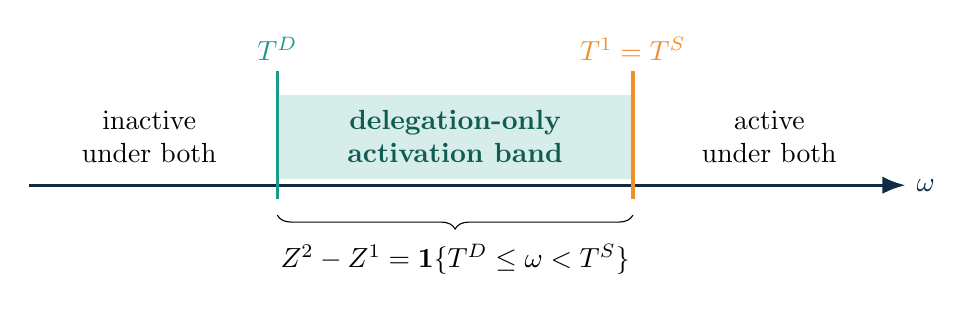
\begin{tikzpicture}[x=1.05cm,y=1cm,>=Latex]
    \draw[->,very thick,Navy] (0,0) -- (10.6,0) node[right] {$\omega$};
    \fill[Teal!18] (3.0,0.08) rectangle (7.3,1.15);
    \draw[very thick,Teal] (3.0,-0.18) -- (3.0,1.45) node[above] {$T^D$};
    \draw[very thick,Orange] (7.3,-0.18) -- (7.3,1.45) node[above] {$T^1=T^S$};
    \node[align=center] at (1.45,.62) {inactive\\under both};
    \node[align=center,text=Teal!60!black,font=\bfseries] at (5.15,.62) {delegation-only\\activation band};
    \node[align=center] at (8.95,.62) {active\\under both};
    \draw[decorate,decoration={brace,mirror,amplitude=5pt}] (3,-.38)--(7.3,-.38);
    \node[below] at (5.15,-.62) {$Z^2-Z^1=\mathbf1\{T^D\le\omega<T^S\}$};
  \end{tikzpicture}
  \vspace{0.35cm}
  \begin{columns}[T,onlytextwidth]
    \column{0.47\textwidth}
      \key{Proposition 1:} menu inclusion gives \(Z^2\ge Z^1\) path by path.
    \column{0.49\textwidth}
      \key{Proposition 2:} with \(B>0\) and continuous \(F\), activation probability is \(F(T^S)-F(T^D)\ge0\).
  \end{columns}
  \source{Quispe and Xu, Section 4.2, Propositions 1-2, pp. 15-16.}
\end{frame}

% 7
\begin{frame}{The stock can keep growing after the first-use flow peaks}
  \textbf{Proposition 3:}
  \[
  \Delta C_i(s)=\sum_{k\in\mathcal U_i}
  \left[(1-p^1_{ik})^{s+1}-(1-p^2_{ik})^{s+1}\right]\ge0.
  \]
  \begin{columns}[T,onlytextwidth]
    \column{0.48\textwidth}
      \begin{block}{Flow}
        Newly used languages can spike at adoption and then fall as the at-risk set is depleted.
      \end{block}
    \column{0.48\textwidth}
      \begin{block}{Stock}
        Cumulative languages retain first uses, so the gap can continue to rise.
      \end{block}
  \end{columns}
  \vspace{0.25cm}
  \warn{Printed strict claim:} under \(p^1=0<p^2\), the paper states strict increase and concavity over the observed horizon. The allowed endpoint \(p^2=1\) breaks both strict inequalities.
  \source{Quispe and Xu, Section 4.3, Proposition 3, p. 17; Theory Appendix proof.}
\end{frame}

% 8
\begin{frame}{At adoption, language breadth rises sharply}
  \begin{columns}[T,onlytextwidth]
    \column{0.57\textwidth}
      \renewcommand{\arraystretch}{1.28}
      \begin{tabular}{lrr}
        \toprule
        Outcome & \(ATT(0)\) & SE \\
        \midrule
        Active languages & \textbf{+2.528} & 0.063 \\
        Newly used languages & \textbf{+1.193} & 0.051 \\
        Language entropy & \textbf{+0.382} & 0.009 \\
        Cumulative languages & \textbf{+1.604} & 0.054 \\
        \bottomrule
      \end{tabular}
      \vspace{0.35cm}

      \small 5,346 developers; 28 months; 3.15 million commits; 57.2 million changed files.
    \column{0.39\textwidth}
      \begin{block}{Economic magnitude}
        Pre-adoption active-language mean: \textbf{0.90}. The active set roughly triples on impact.
      \end{block}
      \vspace{0.2cm}
      The cumulative series has non-trivial pre-trends and is treated as descriptive.
  \end{columns}
  \source{Quispe and Xu, Sections 5 and 7; Table 2; source table \texttt{table\_cl\_main.tex}.}
\end{frame}

% 9
\begin{frame}{The event study does not identify causality}
  \centering
  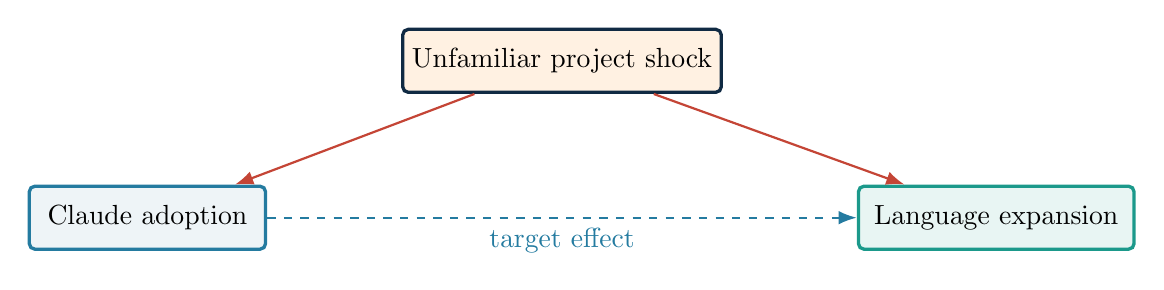
\begin{tikzpicture}[node distance=1.15cm and 1.7cm,>=Latex]
    \node[draw=Navy,very thick,rounded corners=2pt,fill=LightOrange,minimum width=3.2cm,minimum height=.8cm] (shock) {Unfamiliar project shock};
    \node[draw=Blue,very thick,rounded corners=2pt,fill=Mist,below left=of shock,minimum width=3.0cm,minimum height=.8cm] (adopt) {Claude adoption};
    \node[draw=Teal,very thick,rounded corners=2pt,fill=Teal!10,below right=of shock,minimum width=3.5cm,minimum height=.8cm] (frontier) {Language expansion};
    \draw[->,thick,Red] (shock) -- (adopt);
    \draw[->,thick,Red] (shock) -- (frontier);
    \draw[->,thick,Blue,dashed] (adopt) -- node[below,sloped]{target effect} (frontier);
  \end{tikzpicture}
  \vspace{0.22cm}
  \small
  \begin{itemize}\setlength\itemsep{0.12cm}
    \item Staggered DiD handles cohort heterogeneity and avoids already-treated comparisons.
    \item Removing Claude commits and the first-Claude language addresses mechanical measurement.
    \item Neither resolves project-driven adoption; activity already rises at \(e=-1\).
  \end{itemize}
  \warn{Conclusion:} robust event-time associations consistent with delegation, not a causal estimate.
  \source{Quispe and Xu, Section 9, “Discussion: Identification Threats.”}
\end{frame}

% 10
\begin{frame}{AI primitives imply expansion or deskilling}
  \begin{columns}[T,onlytextwidth]
    \column{0.49\textwidth}
      {\color{Teal}\large\textbf{Quispe and Xu}}\par\smallskip
      AI adds specification and delegated execution:
      \[
        \{S,C\}\longrightarrow\{S,C,D\}.
      \]
      A lower threshold activates unfamiliar-language opportunities: the extensive margin expands.

    \column{0.02\textwidth}
      \centering\color{gray!45}\rule{0.4pt}{5.0cm}

    \column{0.49\textwidth}
      {\color{Orange}\large\textbf{Aouad, Lykouris, and Zhong}}\par\smallskip
      Skill, effort, and AI assistance are substitutable inputs:
      \[
        x=s+e+a,\qquad \max_{e\ge0}p(x)-\gamma e.
      \]
      More AI can reduce effort; with endogenous skill or unreliable assistance, productivity can fall and skills can polarize.
  \end{columns}
  \vspace{0.12cm}
  \small\key{Modeling contrast:} menu expansion creates a feasible margin; input substitution can cannibalize effort and skill formation.
  \source{Quispe and Xu, Sections 1 and 4; Aouad, Lykouris, and Zhong (2026), Sections 1-5, arXiv:2605.11350v1.}
\end{frame}

% 11
\begin{frame}{Lean requires \(p_2<1\) for strict dynamics}
  \small
  \textbf{Printed:}\quad
  \(p_1=0<p_2\le1\Rightarrow G_s<G_{s+1}\) and \(\Delta^2G_s<0\).\qquad
  \warn{But at \(p_2=1\):} \(G_s=1-(1-1)^{s+1}=1\).

  \vspace{0.20cm}
  \begin{columns}[T,onlytextwidth]
    \column{0.50\textwidth}
      \textbf{Corrected Spec boundary}\par\smallskip
      \begin{block}{}
      \ttfamily\fontsize{9.3}{11}\selectfont
      \resizebox{\linewidth}{!}{dynamicCumulativeLanguageEffectCorrectedSpec}\\[3pt]
      \quad 0 <= p1 <= p2 <= 1 -> weakGap\\
      \quad p1 = 0 and 0 < p2 < 1\\
      \qquad -> strictIncrease and strictConcavity
      \end{block}

    \column{0.46\textwidth}
      \textbf{Formal refutation}\par\smallskip
      \begin{block}{}
      \ttfamily\fontsize{9.3}{11}\selectfont
      theorem ...EndpointCounterexample :\\
      \quad not ...PrintedStrictClaim := by\\
      \quad intro h\\
      \quad have hUnit := h Unit (fun \_ => 1) ...\\
      \quad have hFalse := hIncreasing 0\\
      \quad norm\_num at hFalse
      \end{block}
  \end{columns}
  \vspace{0.08cm}
  Five endpoints compile with zero `sorry`, `admit`, or axioms; build and `check --fast` succeed. \warn{Verdict: partially formalized.}
  \source{\texttt{lean/PaperInterface.lean}; \texttt{MainTheorems.lean}; \texttt{ProofInterface.lean}; validation report.}
\end{frame}

% 12
\begin{frame}{The handwritten check makes saturation visible}
  \begin{columns}[T,onlytextwidth]
    \column{0.60\textwidth}
      \centering
      \IfFileExists{hand/prop3-endpoint.png}{%
        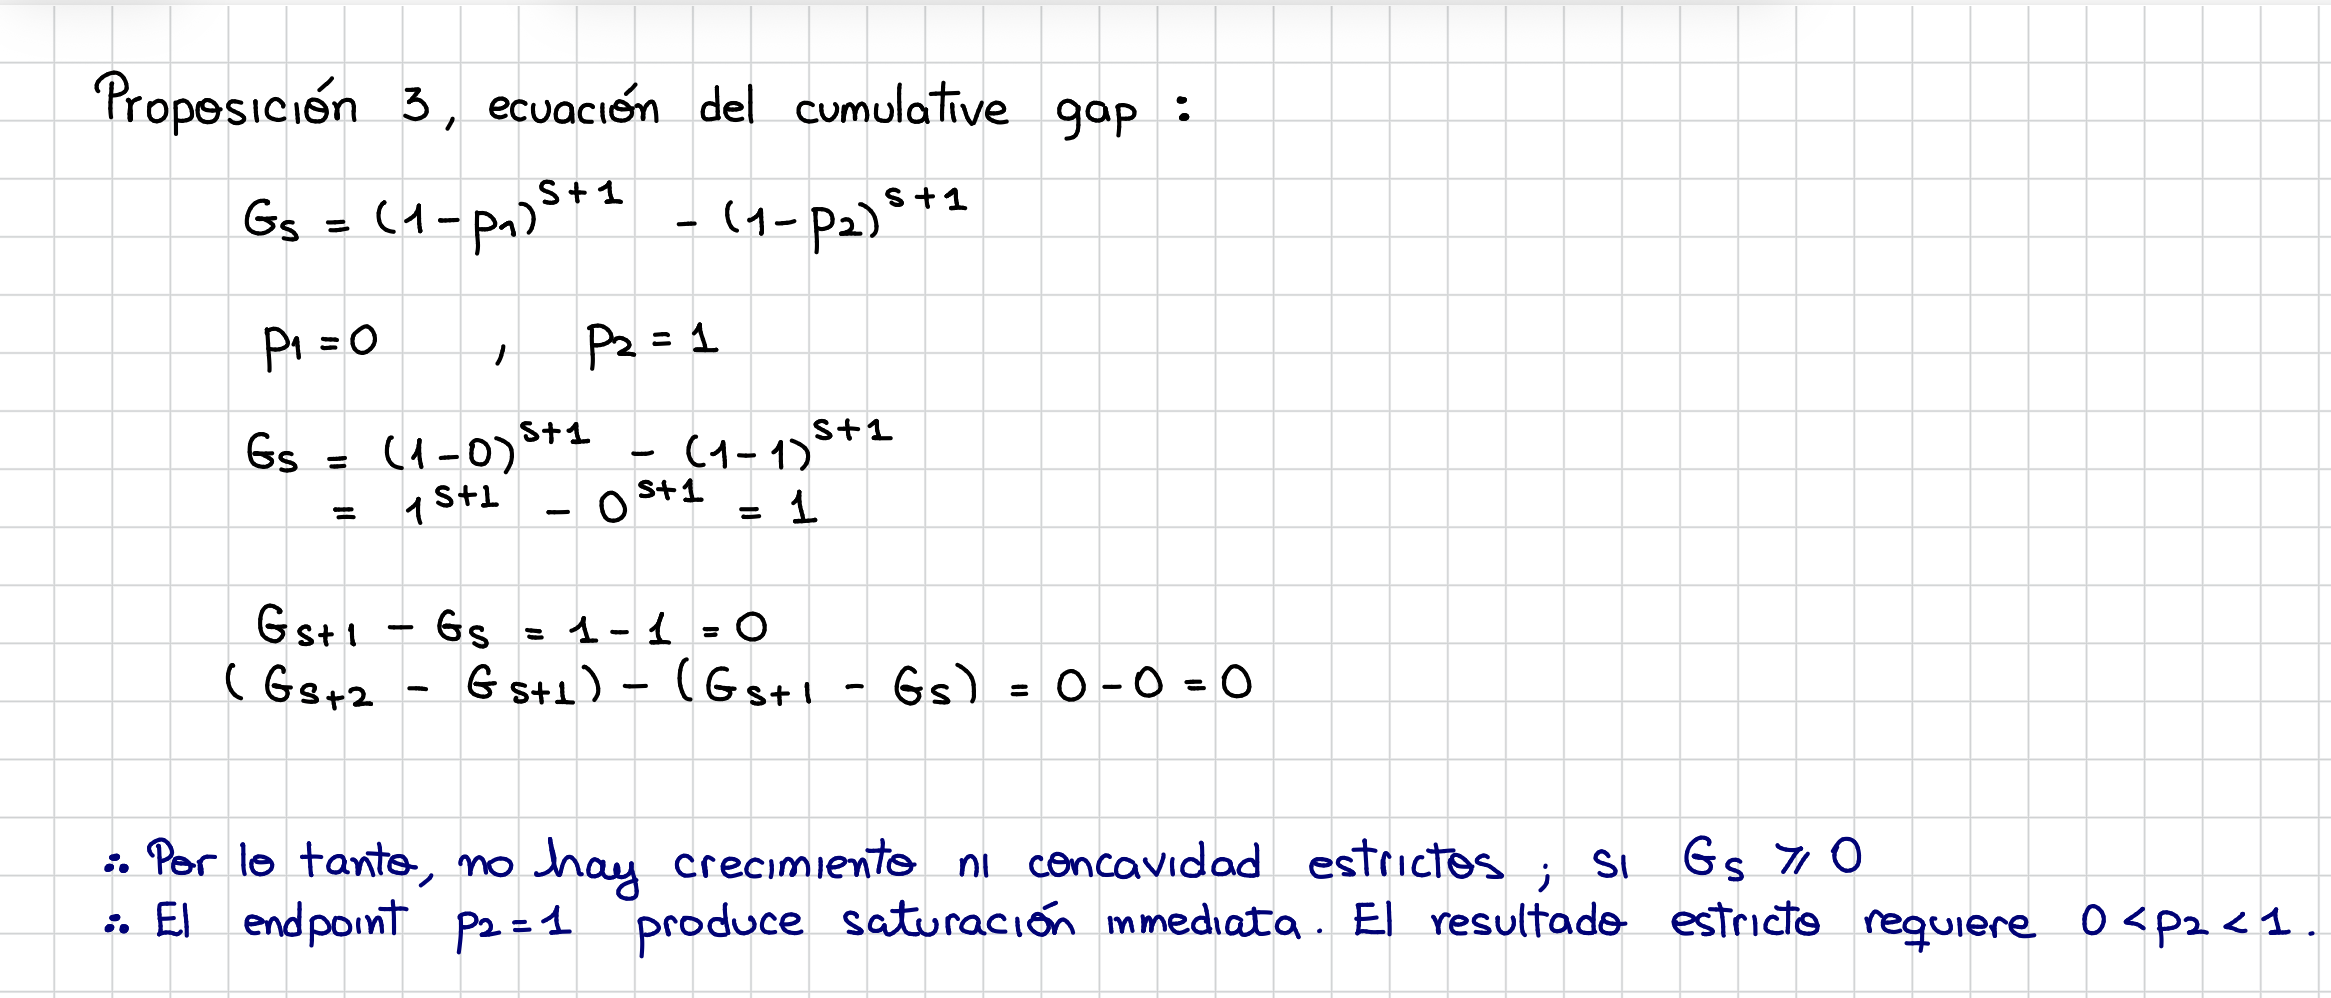
\includegraphics[width=\linewidth,height=0.69\textheight,keepaspectratio]{hand/prop3-endpoint.png}%
      }{%
        \PackageError{presentation}{Missing hand/prop3-endpoint.png}{The handwritten verification image is required for slide 12}%
      }
    \column{0.36\textwidth}
      \textbf{Two-minute derivation}\par\smallskip
      Set one language, \(p_1=0\), \(p_2=1\). Then show:
      \[
      G_s=(1-0)^{s+1}-(1-1)^{s+1}=1.
      \]
      Hence \(G_{s+1}-G_s=0\), contradicting strict growth; the second difference is also zero.
  \end{columns}
  \source{Quispe and Xu, Proposition 3 and its Theory Appendix proof; independent Lean endpoint audit.}
\end{frame}

% 13
\begin{frame}{Expansion does not uniquely identify delegation}
  \begin{columns}[T,onlytextwidth]
    \column{0.53\textwidth}
      \textbf{Extension: generic productivity}\par\smallskip
      Replace skill-complementary augmentation with
      \[
        V^P=V^S+q-r_P,\qquad T^P=T^S-(q-r_P).
      \]
      If \(q>r_P\), even a non-agentic shock creates an activation band. Expansion alone does not reveal whether \(T^P\) or \(T^D\) moved.

    \column{0.43\textwidth}
      \textbf{Discriminating test}\par\smallskip
      Cross post-adoption change with:
      \begin{itemize}\setlength\itemsep{0.18cm}
        \item pre-adoption portfolio breadth,
        \item independent verification ability,
        \item task-level delegation intensity.
      \end{itemize}
      Delegation predicts a positive interaction; a common productivity shift does not.
  \end{columns}
  \vspace{0.12cm}
  \small\key{Bottom line:} a large shift in production breadth; five compiled Lean cores; one strict-endpoint defect; causal and mechanism-specific identification remain open.
  \source{Quispe and Xu, Theory Appendix and Sections 8-10; extension developed in \texttt{extensions.md}.}
\end{frame}

\end{document}
